\section{Classification Algorithms}
\label{section:classification}

To perform activity recognition, there are a variety of machine learning algorithms to consider. The ones used in this study are decision tree, k-nearest neighbor and support vector machine. This chapter aims to provide a detailed explanation for each of them.

All of the algorithms mentioned below are supervised learning models, meaning that they all need a set of input-output pairs. The input typically represents a vector of features, while the output represents the desired classification. This data is used to train the algorithm to generate a function which maps new feature vectors to one of the previously trained classes.


\subsection{Decision Tree}
A decision tree is a structure of nodes. Each node represents either a decision node, a chance node, or an end node. A decision node is a test on a property or feature, and branches off into two or more nodes. These again can be either of the three mentioned nodes. A chance node represents a decision which is based on probability, rather than being fully deterministic. An end node, or leaf node, is the last node of a branch and represents the outcome of the classification. A tree where every node branches off in only two nodes is called a binary decision tree. Every tree that has branches with more than two nodes can be converted into a binary decision tree.

In the case of activity recognition decision nodes represent the different features of each sample, like the magnitude of the acceleration, the direction of the acceleration along the three axes or the time between peaks. Each end node represents an activity the user can perform and which can be recognized, like walking, running or standing.

One of the benefits of decision trees is that they are quite easy to understand. After a short explanation, most people interpret a decision tree. In combination with an \gls{ann}\footnote{An \gls{ann} is a machine learning algorithm based on the idea of biological neural networks. It learns to perform tasks without prior knowledge, which also affect the structure of the \gls{ann}.}, it is possible to add new possible branches and outcomes, or just replace inefficient branches. This makes it suitable as a machine learning algorithm, since it can start developing its own branches and adjust already existing ones on its own.

Its main drawback is that they are relatively unstable, meaning that a decision tree might have to be heavily restructured when small changes to the data are made. This can mitigate a lot of prior work. Additionally they often tend to be quite inaccurate. Usually a decision tree yields worse results concerning accuracy and prediction, when compared to other classification algorithms. This is caused by its discrete decision making nature \autocite[]{king1995statlog, gascuel1998twelve}, as will be confirmed later in chapter \ref{section:results}. This gets alleviated by the fact that a decision tree can be combined with other machine learning algorithms. This way its performance can be improved and its accuracy can be increased. This is not investigated further during this study though.


\subsection{Nearest Neighbors}
The nearest neighbor algorithm is an algorithm which classifies data based on a nearest neighbor rule. When it is using the \gls{1nn} rule, the algorithm looks for the closest sample of a training set and will choose the same classification as the closest training sample it finds. In contrast the \gls{knn} rule does not only look for the closest training sample, but the K closest samples and chooses a classification based on a majority vote \autocite[]{cover1967nearest}.

There are different approaches for deciding which neighbors should be taken into consideration. The simplest and most straight forward way is to assign a class by majority decision. The more neighbors belong to the same class, the more likely it is, that the new sample belongs to the same class. Additionally a distance function could be implemented, giving neighbors which are closer to your sample more weight during the classification.

\begin{figure}[!ht]
    \centering
    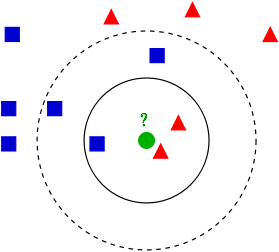
\includegraphics[width=0.5\linewidth]{images/Classification-Knn.png}
    \caption[]{
        K-Nearest Neighbor Classification \autocite[]{image-knn}
    }
    \label{figure:knn}
\end{figure}

It is oftentimes preferred to use \gls{knn} over \gls{1nn}. It takes more computational time, but especially in areas where samples tend to overlap and distinctions are not as clear, it improves the probability of a correct classification as it reduces the effect of noise \autocite[]{clusterAnalysis}. Therefore choosing a reasonable value for K is important. If K is too big, a lot of data has to be processed, and room for error is generated, since more neighbors of wrong classes could be taken into consideration. If K is too small though, noise may cause wrong classification as well. In figure \ref{figure:knn} a classification via \gls{1nn} would suggest that the green dot belongs to the class of red triangles. By using \gls{knn} with K = 5 the algorithm would determine that the green dot instead belongs to the blue squares. Which value is appropriate depends on the experiment and the desired outcome. As elaborated, this is an important part of the testing process.


\subsection{Support Vector Machine}
A previously mentioned, a \gls{svm} is a supervised learning model, which tries to find a hyper-plane\footnote{A hyper-plane is a geometrical subspace that has one less dimension than its ambient space. It separated the space into two half-spaces.}, that separates the different classes. The space between the samples of the training data and the hyper-plane has to be maximized. Depending on their position and distance relative to the hyper-plane new samples can be classified as either one of the two possible classes. This version of a \gls{svm} is called a Linear \gls{svm}. An example of this is shown in figure \ref{figure:svm}.

\begin{figure}[!ht]
    \centering
    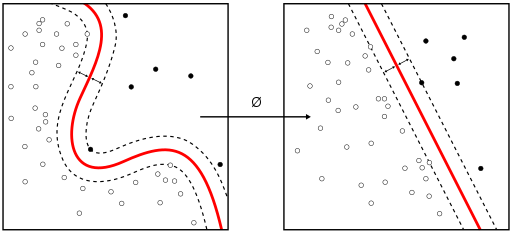
\includegraphics[width=0.75\linewidth]{images/Classification-Svm.png}
    \caption[]{
        Support Vector Machine Classification \autocite[]{image-svm}
    }
    \label{figure:svm}
\end{figure}

One upside of this algorithm is that not all training samples need to be considered for the generation of the hyper-plane. Samples which are surrounded by samples of the same class, or are further away from the plane, have no influence on the plane. This makes the computation a bit easier. The samples closest to the plane are stored as so-called support vectors, since they are sufficient to describe the hyper-plane.

A lot of times the sets of data are not linearly separable in their original space. This is often the case when there are more than two possible classifications. To approach a problem like this, kernel functions are used. These transform the data set into a higher dimensional space. At one point, if the number of dimensions is high enough, the data set will be linearly separable again by fitting a set of hyper-planes in this higher dimensional space \autocite[]{vert2004primer}.

Transformations like these are quite demanding, so transforming every sample into this higher dimensional space is not feasible. This is where the \textit{kernel trick} comes into play \autocite[]{vert2004primer}. By choosing the right kernel functions, the transformation becomes a lot easier. The effect of these kernel functions is that dot products can be computed very easily in both spaces, which equals the distance between the sample and the hyper-planes. This property is used to classify samples when using a \gls{svm}.

Examples of kernel functions for nonlinear \gls{svm} are a polynomial kernel and \gls{rbf}. These functions replace the dot product, when calculating the distance of each sample to the hyper-planes, with a function, that represents a distance function in a higher dimensional space \autocite{vert2004primer}.

A polynomial kernel (\ref{equation:polynomial-kernel}) can either be in-homogeneous or homogeneous if $c = 0$. The parameter $c$ is adding weight to either higher-order or lower-order terms in the polynomial.

\begin{equation}
    K_{poly}(\vec{x_{i}},\vec{x_{j}})=(\vec{x_{i}}\cdot\vec{x_{j}}+c)^{d}
    \label{equation:polynomial-kernel}
\end{equation}

An \gls{rbf} (\ref{equation:rbf-kernel}) is one of the most frequently used kernels in classification problems when using a \gls{svm}. It has a lot of favorable characteristics, like being able to generate non-parametric classification functions. Therefore almost any decision boundary can be obtained with this kernel. $\sigma$ is a parameter to tweak the kernel function. Smaller values lead to more complex decision boundaries, while larger ones will result in a smoother decision boundary \autocite{vert2004primer}.

\begin{equation}
    K_{rbf}(\vec{x_{i}},\vec{x_{j}})=\mathrm{exp}(-\frac{\left\|\vec{x_{i}}-\vec{x_{j}}\right\|^2}{2\sigma^{2}})
    \label{equation:rbf-kernel}
\end{equation}

While it is also possible to create and use custom kernel functions, it is not part of this study and will not be elaborated any further.
